\section{Filtering Documents} \label{sec:filtering_docs}
Because not all data from information sources such as Common Crawl is relevant to find relationships between cities, the data needs to be filtered. One way to do this, is to only select the data that mentions at least two different cities. Because the data is plain text, we need a way to scan through the text and determine if the text indeed has a co-occurrence of two different cities.
Making use of the comparative analysis of Rasool et al. \cite{rasool2012string}, we chose the Aho-Corasick algorithm \cite{Aho-Corasick}, which is a multi-pattern exact string matching algorithm and is the driver of widely used tools such as \texttt{grep} \cite{kernighan1984unix}. The algorithm creates a finite state machine, where strings to match are final states. Since we are looking for the co-occurrence of cities, using a multi-pattern string matching algorithm is preferred over a plain string matching algorithm. This is especially well illustrated by table \ref{tab:bm-matching} below. The benchmark was performed on a string of 1500 characters, with a million iterations. In the table, the average speed of matching is shown in milliseconds.

\begin{table}[H]
\centering
\begin{tabular}{ |c|c| } 
    \hline
    multi-pattern matching & 0.049831339 \\
    plain string matching &  1.870154497 \\
    \hline
\end{tabular}
\caption{Benchmark of multi-string vs. plain string matching}
\label{tab:bm-matching}
\end{table}

The decision to use the Aho-Corasick algorithm is strengthened by the fact that a well documented and stable Python library exists, which implements the aforementioned algorithm. This library is called \texttt{pyahocorasick}\footnote{\url{https://pypi.python.org/pypi/pyahocorasick/}} and is a fast and memory efficient implementation of the Aho-Corasick algorithm.

Using the Aho-Corasick algorithm, a predefined list of cities can be matched against the text of a web page or document. If at least two cities from the list appear in the text, we mark it as a useful document. However, an interesting note is that there are pages with lists of cities contained, e.g. to let users select their place of birth. These hardly represent intercity relations, so a maximum of 25 unique occurrences is used to cancel as much of those lists as possible beforehand. The threshold is decided upon by the client, after having analysed figure \ref{fig:occ_per_page} and documents with 20 to 25 unique occurrences.

\begin{figure}[H]
    \centering
    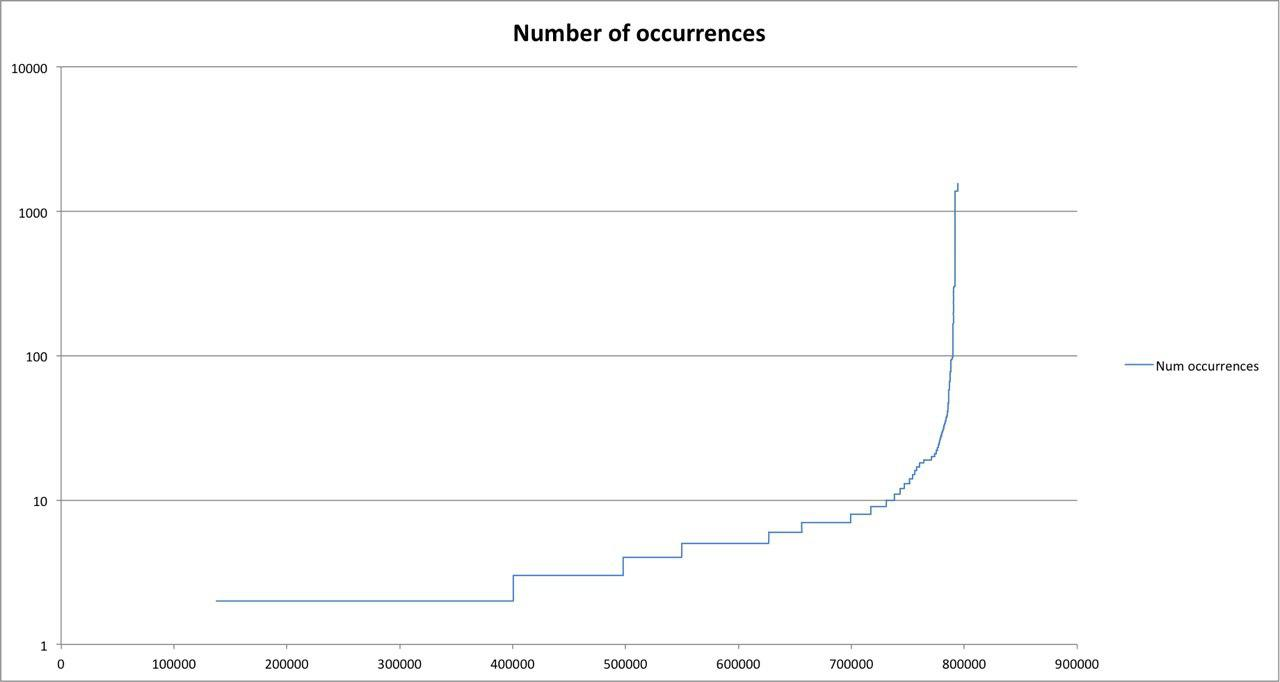
\includegraphics[width=0.8\textwidth]{occurences_per_page}
    \caption{Number of documents plotted against the number of unique occurrences contained in these documents.}
    \label{fig:occ_per_page}
\end{figure}

We make a selection of documents without storing the documents first, because storing all documents is not feasible due to storage constraints. For the .nl web pages only would need about 250GB of storage and to store all available documents around 250TB of storage would be needed. As we do not have access to a fast and large data storage platform, we will not store everything first and then delete documents that were filtered out. However, to test if finding and storing relationships between cities is fast enough when the documents are actually stored on disk, a random selection of 1 million documents will be downloaded. Processing the already stored documents could finish within one day\footnote{On a virtual server with 8GB RAM, 4 CPUs and 100GB of HDD storage.} whereas downloading all documents will most certainly take multiple days.


% \todo{add info:}

% Piet Bep, [16.06.17 11:55]
% num 20
% 773665
% num 30
% 7510
% num 40
% 4020
% num 50
% 979

% Piet Bep, [16.06.17 11:55]
% bovenstaande is aantal documenten met minder dan 20 occurrences, tussen 20 en 30, tussen 30 en 40, en tussen 40 en 50